




\tightsection{Evaluation}
\label{sec:eval}

In this section, we evaluate the performance of the GO system in real-world. Based on the observation from running GO on one content provider, 
\begin{packedenumerate}
    \item We see an overall 7\% reduction in buffering ratio, 4\% increase in average bitrate, and 16\% reduction in number of bitrate switches.
    \item We see buffering raito reduction of more than 20\% in one day when a major CDN is experiencing performance degradation that lasts for about 2 days.
    \item We show that the initial bitrate chosen by GO is 19\% closer to the dominant bitrate.
\end{packedenumerate}

\tightsubsection{Setup}
\label{subsec:eval_setup}

We evaluate the performance of GO on one content provider with short-form videos (5 minutes) on iOS device (both iPhone and iPad). 
HLS protocol is running on the iOS device and our GO system provides the initial CDN and bitrate, while Apple player employs adaptive 
bitrate switching algorithm. 

There are three CDNs in this experiement, and 5 bitrate levels (from 700Kbps to 3.5Mbps). We evaluate two algorithms: {\it randomized} 
and {\it optimized} (by GO).

\tightsubsection{Rebuffering Rate and Average Bitrate}

Figure~\ref{subfig:buffering-and-bitrate} shows the performance improvement of optimized over randomized algorithm. Performance improvement varies by time,
depending on how stable performance of CDN is. On day 30, we noticed a big performance improvement of more than 20\%,
it turns out a major CDN was experiencing performance issues that lasts for more than one day. Table XXX shows the 
performance and decisions, and indicates that GO can respond to such events and adjust decisions accordingly.

\begin{figure*}[t!]
\centering
\subfigure[Rebuffering ratio and average bitrate]
{
  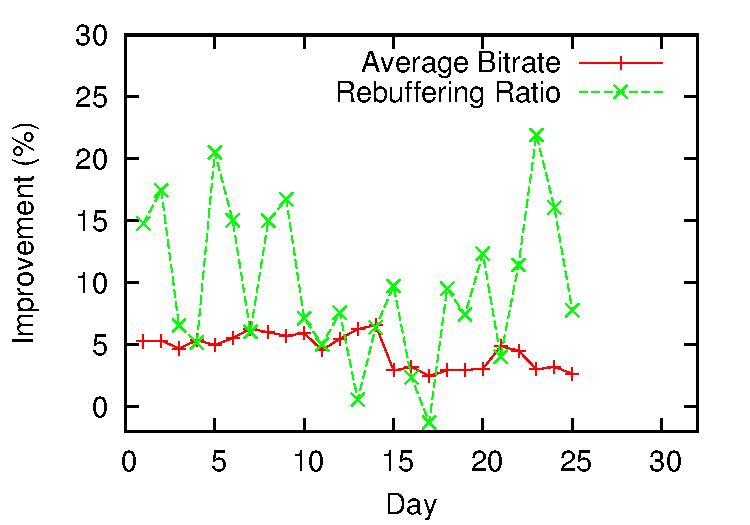
\includegraphics[width=0.3\textwidth] {figures/eval-perfimp.pdf}
  \label{subfig:buffering-and-bitrate}
}
\subfigure[Number of bitrate switches]
{
  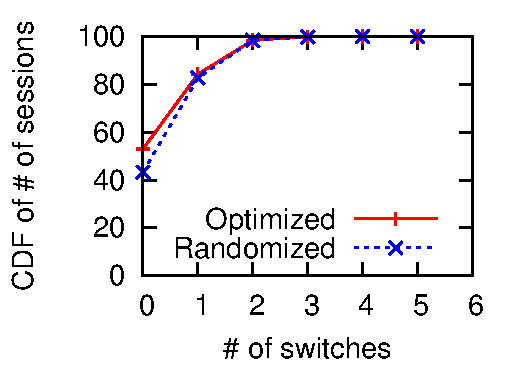
\includegraphics[width=0.3\textwidth] {figures/eval-reduceswitch.pdf}
  \label{subfig:reduce-switch}
}
\subfigure[Initial vs. dominant bitrate]
{
  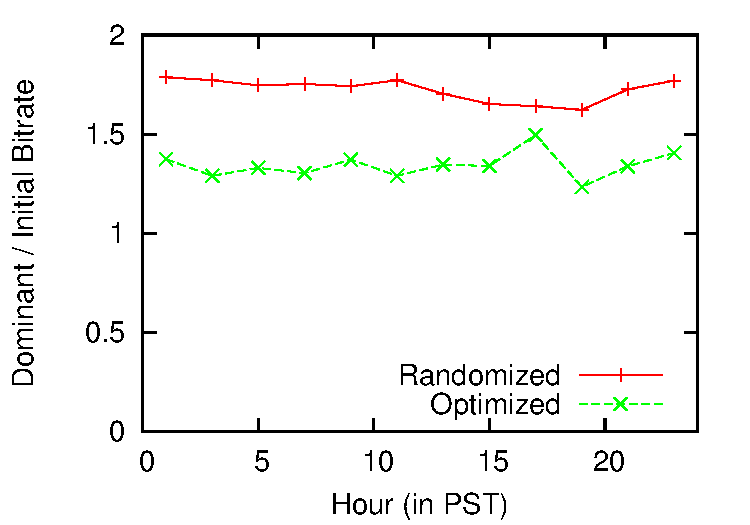
\includegraphics[width=0.3\textwidth] {figures/eval-initvsdom.pdf}
  \label{subfig:initvsdom}
}
\tightcaption{Performance Metrics and Improvement from GO}
\label{fig:perf-impr}
\end{figure*}


\subsubsection{Case study}
Now we look into some particular example and see how GO improves quality by allocating traffic to best CDN. Figure~\ref{fig:eval-case-study} shows three example days in which three CDNs performed differently: in terms of average bitrate and buffering ratio, CDN1 was the best on Day A, CDN2 was the best on Day B and three CDNs performed similarly on Day C. We can see that in both Day A and B, GO managed to allocate more traffic to the best CDN (Figure~\ref{subfig:eval-case-study:share}) and maintain the global average quality to be similar to the best CDN in both average bitrate and buffering ratio. Even on Day C, GO still managed to reach an arguably improvement of buffering ratio and average bitrate. This indirectly suggests that GO was not only looking for the globally best CDN, but also differentiated CDN performance in finer granular partition.


\begin{figure*}[t!]
\centering
\subfigure[Buffering ratio]
{
	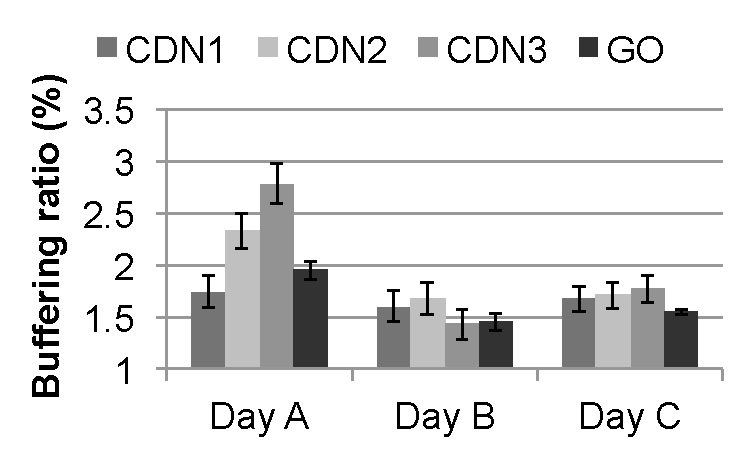
\includegraphics[width=0.3\textwidth]{figures/ab-testing-figures/bufferingratio.pdf}
	\label{subfig:eval-case-study:bufferingratio}
}
\subfigure[Average bitrate (Kbps)]
{
	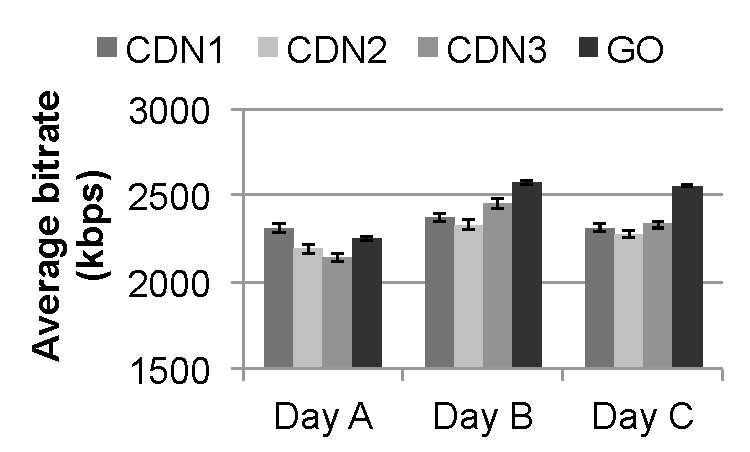
\includegraphics[width=0.3\textwidth]{figures/ab-testing-figures/averagebitrate.pdf}
	\label{subfig:eval-case-study:averagebitrate}
}
\subfigure[Traffic share of different CDNs]
{
	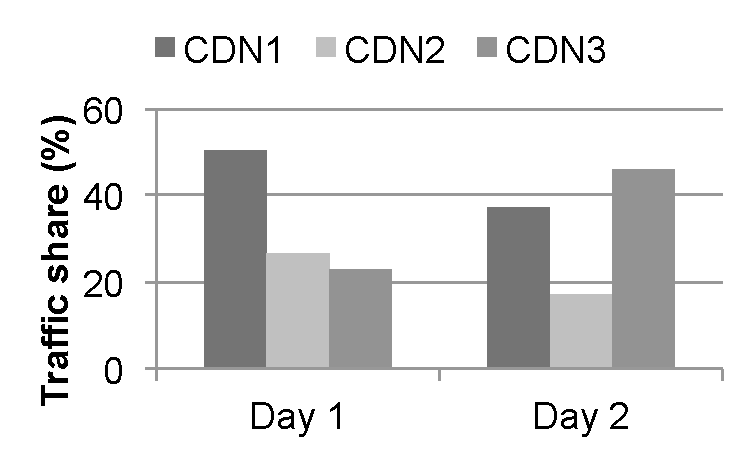
\includegraphics[width=0.3\textwidth]{figures/ab-testing-figures/trafficshares.pdf}
	\label{subfig:eval-case-study:share}
}
\tightcaption{Case study of three days: CDN1 was the best on Day A and CDN2 was the best on Day B. In both cases, GO managed to allocate more traffic to the best CDN and maintain the global average quality to be similar to the best CDN in both average bitrate and buffering ratio. Even on Day C where three CDN performed similarly, GO still managed to reach an arguably improvement of buffering ratio and average bitrate.}
\label{fig:eval-case-study}
\end{figure*}



\tightsubsection{Adaptive Bitrate Stability}

\tightsubsubsection{When Do Adaptive Bitrate Switches Happen?}

Figure~\ref{fig:switch-time-dist} shows when do adaptive bitrate switches happen. To account for viewers leaving in the middle 
of the video play, the x-axis is chosen as the percentage of actual video play duration instead of content length. 
In this figure, we include another content provider who provides long-formed content on iOS platforms.

The figure shows that the majority of switches happen at the beginning of the video plays, i.e., around 60\% of the switches 
happen within 20\% of the video duration. Switching behavior varies for different adaptive bitrate algorithms, and we do not 
claim such observation apply to all algorithms.

This suggests the importance of initial bitrate selection, through which viewers can have a smoother video playback experience.

\begin{figure}[h!]
\centering
 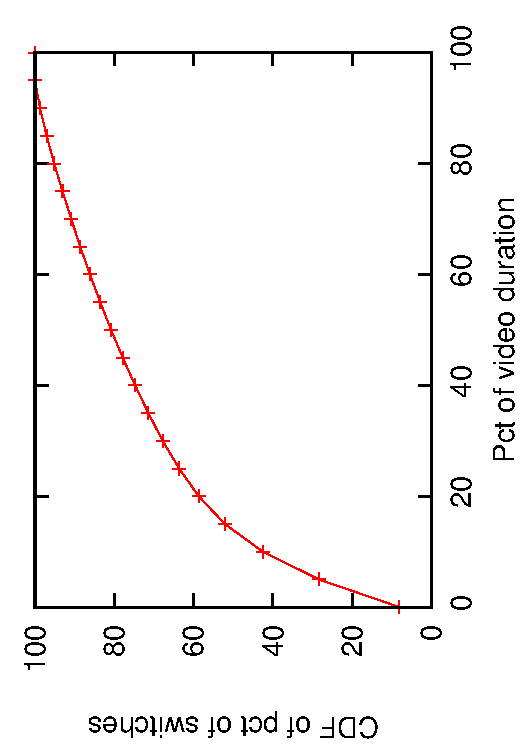
\includegraphics[width=0.4\textwidth] {figures/switch-time-dist.pdf}
\tightcaption{When Do Adaptive Bitrate Switches Happen}
\label{fig:switch-time-dist}
\end{figure}

\tightsubsubsection{Reducing Number of Bitrate Switch}

Figure~\ref{subfig:reduce-switch} shows the number of bitrate switches for optimized and random decisions within the first minute. 
It shows that GO can reduce the number of switches.

\tightsubsubsection{Initial vs. Dominant Bitrate}

Figure~\ref{subfig:initvsdom} shows the ratio of initial bitrate to dominant bitrate (1 is best). It shows that GO is close to dominant bitrate.
